\newpage
\section{Praktikum 3 - Teil I: Fortgeschrittenes Reporting und Dokumentähnlichkeit auf zerlegten Texten (SQL)}

\subsection{Bigramme}

\begin{center}
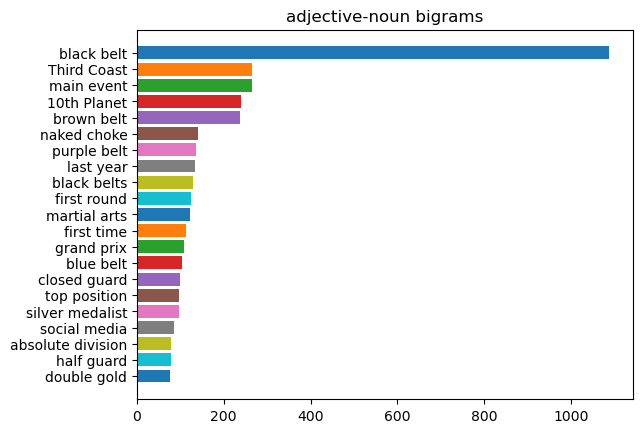
\includegraphics[width=0.6\textwidth]{images/adj_noun_bigrams.png}
\end{center}

\noindent Dass der Schwarzgurt alle anderen Adjektiv-Nomen Bigramme so stark abhängt war etwas überraschend. Auch andere Gurte sind vertreten (\texttt{black/brown/purple/blue}), interessanterweise in Reihenfolge vom höchstgradierten bis niedrigstgradierten, mit Ausnahme des wei{\ss}en Gurtes, welcher der Anfänger Gürtel ist und in absoluter Anzahl die meisten Teilnehmer ausmacht. Das Interesse scheint demnach stark auf den Wettkämpfen und sozialem Drama der \texttt{black belt} Klasse zu liegen. Die Adjektive der \texttt{main event, first round, first time} waren zu erwarten. Das Erste oder der Hauptteil sind von besonderem Interesse. \texttt{10th Planet} ist eine gro{\ss}e Organisation im No-Gi Submission Grappling, worauf die Webseite einen Fokus legt gegenüber Gi Grappling. \texttt{naked choke, closed guard, top position, half guard} sind zentrale Positionen und Techniken aus dem BJJ.

\subsection{Co-occurences}

\begin{center}
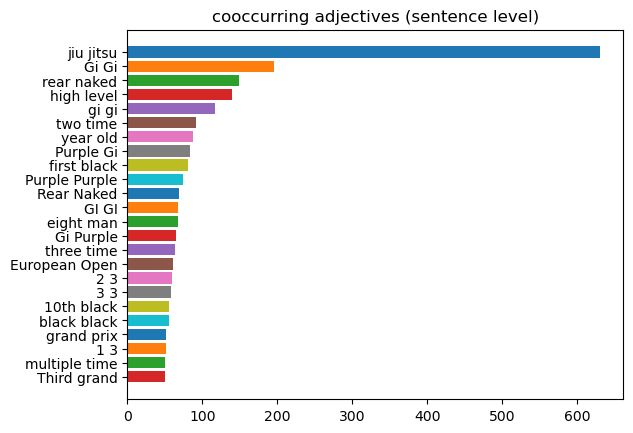
\includegraphics[width=0.6\textwidth]{images/coocc_adj.png}
\end{center}

\noindent \texttt{jiu jitsu, Gi Gi, gi gi, Purple Gi, Purple Purple, GI GI, 2 3, 3 3, black black, 1 3} ist unsinniger Output, der aus einer falschen TA\_TYPE bestimmung stammt. \\

\noindent \texttt{rear naked, Rear Naked} ist wieder Teil der Technik "Rear Naked Choke", wobei die adjektiv Kombination \texttt{rear naked} alleinstehend im Grappling Kontext lustige Bilder hervorruft. \texttt{high level, two time, year old, first black, three time, European Open, grand prix, multiple time, third grand} sind alle sehr passend zu einem Wettkampf Kontext. Die Seite scheint wirklich besonders darüber zu berichten.

\subsection{tf-idf}

{\color{MidnightBlue}
\begin{lstlisting}
word: box, url: https://grapplinginsider.com/the-bjj-box-why-you-should-buy-one/
tf-df: 48.17, tf: 29, idf: 1.66

word: rib, url: https://grapplinginsider.com/rib-injuries-in-bjj-causes-diagnosis-and-prevention/
tf-df: 47.46, tf: 30, idf: 1.58

word: pounds, url: https://grapplinginsider.com/nogi-worlds-competitor-list-and-preview/
tf-df: 41.02, tf: 30, idf: 1.37
\end{lstlisting}}

\noindent Das sind alles Worte die in den Dokumenten sehr häufig vorkommen (tf), aber im Corpus nahezu garnicht (idf). Die Dokumente handeln sehr zentral von diesen Worten. Bei letzterem nur indirekt, aber \texttt{pound} wird in dieser 'competitor list' häufig gelistet. Dass aufgrund des \textit{ntn} Schemas nach SMART Notation keine Normalisierung stattfand war nicht von besonderer Bedeutung, da die Dokumente nicht viel länger sind als andere.

\subsection{similarity}

{\color{MidnightBlue}
\begin{lstlisting}[language=python]
def get_similar(self, target_url, n=10, mode="cos"):  # modes = ["scalar", "cos"]
    command = """
    SELECT URL, TA_TOKEN
    FROM "$TA_GRAPPLING_INSIDER_INDEX"
    WHERE TA_TYPE = 'noun'
    ORDER BY URL ASC
    """
    self.cursor.execute(command)
    # create data
    vecs_dict = {}
    for res in self.cursor:
        url = res[0]
        noun = res[1]
        if url not in vecs_dict:
            vecs_dict[url] = {}
        if noun in vecs_dict[url]:
            vecs_dict[url][noun] += 1
        else:
            vecs_dict[url][noun] = 1
    data = pd.DataFrame(vecs_dict)
    data = data.fillna(0)
    data = data.astype(int)
    data = data.transpose()
    # get vec
    vec = data[data.index == target_url]
    # determine similarity
    if mode == "scalar":
        data["sim"] = data.apply(lambda row: sum(row.values*vec.values[0]), axis=1)
    elif mode == "cos":
        data["sim"] = data.apply(lambda row: sum(row.values*vec.values[0])/
            sqrt(sum(row.values**2))*sqrt(sum(vec.values[0]**2)), axis=1)
    else:
        print("unknown mode")
        return None
    # sort by similarity
    data = data.sort_values("sim", ascending=False)
    # return top n urls
    return list(data.index)[1:n+1]
\end{lstlisting}}

\subsection{similarity prüfen}

\noindent- input: \\
{\color{MidnightBlue}
\url{https://grapplinginsider.com/john-danaher-picks-the-best-open-guard/}} \\
\noindent- output: \\
{\color{MidnightBlue}
\url{https://grapplinginsider.com/gordon-ryan-explains-how-to-improve-your-butterfly-and-open-guard/}, \\
\url{https://grapplinginsider.com/wno-ryan-vs-diniz-full-card-play-by-play/}, \\
\url{https://grapplinginsider.com/john-danaher-details-his-systematic-approach-to-no-gi-guard-passing/}, \\
\url{https://grapplinginsider.com/gordon-ryans-half-guard-instructional-dropping-soon/}, \\
\url{https://grapplinginsider.com/polaris-11-results-play-by-play/}, \\
\url{https://grapplinginsider.com/third-coast-grappling-kumite-vi-review-hugo-wins/}, \\
\url{https://grapplinginsider.com/learn-the-seven-most-simple-guard-passes/}, \\
\url{https://grapplinginsider.com/xande-ribeiro-explains-the-side-closed-guard/}, \\
\url{https://grapplinginsider.com/combat-jiu-jitsu-worlds-the-middleweights-results/}, \\
\url{https://grapplinginsider.com/no-gi-worlds-2019-results-adam-wardzinski-sets-biggest-points-difference-of-the-day/}} \\

\noindent$\Rightarrow$ John Danaher ist der Trainer von Gordon Ryan. Die ähnlichen Artikel handeln häufig über Technik Informationen die diese beiden geben. Es sind auch einige Artikel über Wettkämpfe dabei. \\

\noindent- input: \\
{\color{MidnightBlue}
\url{https://grapplinginsider.com/ryan-hall-still-cant-get-anyone-to-fight-him/}} \\
\noindent- output: \\
{\color{MidnightBlue}
\url{https://grapplinginsider.com/breaking-conor-mcgregor-v-donald-cowboy-cerrone-official-for-ufc-246/} \\
\url{https://grapplinginsider.com/watch-every-kneebar-finish-in-ufc-history/} \\
\url{https://grapplinginsider.com/khabib-nurmagomedov-v-tony-ferguson-is-on/} \\
\url{https://grapplinginsider.com/video-bj-penn-involved-in-second-bar-brawl-this-year/} \\
\url{https://grapplinginsider.com/rener-gracie-recaps-logan-paul-vs-floyd-mayweather-from-jiu-jitsu-perspective/} \\
\url{https://grapplinginsider.com/demian-maia-v-gilbert-burns-in-the-works/} \\
\url{https://grapplinginsider.com/nick-diaz-announces-return-to-mma/} \\
\url{https://grapplinginsider.com/georges-st-pierre-adcc-anderson-silva/} \\
\url{https://grapplinginsider.com/demian-maia-not-ready-to-retire-yet-plans-to-compete-in-jiu-jitsu/} \\
\url{https://grapplinginsider.com/yamauchi-sets-new-record-at-bellator-229/}} \\

\noindent$\Rightarrow$ Ryan Hall ist ein UFC Wettkämpfer. Alle ähnlichen Artikel handeln von UFC Wettkämpfen, allerdings nicht von seinen. \\

\noindent- input: \\
{\color{MidnightBlue}
\url{https://grapplinginsider.com/5-reasons-why-marcelo-garcia-is-the-greatest-of-all-time/}} \\
\noindent- output: \\
{\color{MidnightBlue}
\url{https://grapplinginsider.com/euros-2020-mikey-musumeci-enters-the-openweight-division/} \\
\url{https://grapplinginsider.com/making-the-case-5-reasons-why-roger-gracie-is-the-greatest-of-all-time/} \\
\url{https://grapplinginsider.com/marcus-buchecha-almeida-gle-and-leo-vieira-get-us-citizenship/} \\
\url{https://grapplinginsider.com/exclusive-elisabeth-clay-constant-competitor-won-no-gi-pans-on-likely-torn-mcl/} \\
\url{https://grapplinginsider.com/mo-jassim-adcc-2019-seth-daniels/} \\
\url{https://grapplinginsider.com/wno-championships-preview-will-mikey-musumecis-dominance-continue-at-lightweight/} \\
\url{https://grapplinginsider.com/brianna-ste-marie-we-deserve-just-as-much-of-a-platform-as-the-men/} \\
\url{https://grapplinginsider.com/euros-2020-3-things-to-look-out-for-on-the-final-day/} \\
\url{https://grapplinginsider.com/watch-roger-gracie-v-andre-galvao/} \\
\url{https://grapplinginsider.com/tom-deblass-retirement-reddit-adcc/}} \\

\noindent$\Rightarrow$ Marcelo Garcia ist ein BJJ Wettkämpfer. Es geht um einige andere Wettkämpfer die ebenfalls Veteranen sind und heute im Ruhestand. Es sind auch ein paar aktuelle Wettkämpfe dabei, die ich dem ursprünglichen Artikel nicht zuordnen kann. \\

\noindent- input: \\
{\color{MidnightBlue}
\url{https://grapplinginsider.com/who-has-beaten-more-adcc-medalists-gordon-ryan-or-andre-galvao/}} \\
\noindent- output: \\
{\color{MidnightBlue}
\url{https://grapplinginsider.com/year-end-awards-who-was-the-best-male-no-gi-grappler-in-2021/} \\
\url{https://grapplinginsider.com/year-end-awards-who-was-the-best-female-no-gi-grappler-in-2021/} \\
\url{https://grapplinginsider.com/meet-the-stacked-bjj-stars-v-heavyweight-grand-prix-line-up/} \\
\url{https://grapplinginsider.com/2021-ibjjf-no-gi-worlds-preview-the-loaded-middleweight-division/} \\
\url{https://grapplinginsider.com/demian-maia-to-face-alex-cowboy-oliveira-in-first-grappling-match-since-ufc-release/} \\
\url{https://grapplinginsider.com/bjj-stars-8-previewing-the-loaded-8-man-gi-grand-prix/} \\
\url{https://grapplinginsider.com/2021-ibjjf-pans-preview-the-loaded-featherweight-division/} \\
\url{https://grapplinginsider.com/jessa-khan-to-make-one-championship-debut-against-amanda-tubby-alequin/} \\
\url{https://grapplinginsider.com/diego-pato-oliveira-leaves-cicero-costha-joins-dream-art-project/} \\
\url{https://grapplinginsider.com/andre-galvao-inducted-into-the-adcc-hall-of-fame/}} \\

\noindent$\Rightarrow$ ADCC sind quasi die Olympischen Spiele des No-Gi Submission Grapplings. Alle ähnlichen Artikel handeln ebenfalls von No-Gi Submission Grappling. Es schleichen sich kleine Ausnahmen wie ein UFC Match ein.

\setcounter{section}{2}
\section{Praktikum 3 - Teil II: Evaluation}

\subsection{similarity precision/recall}

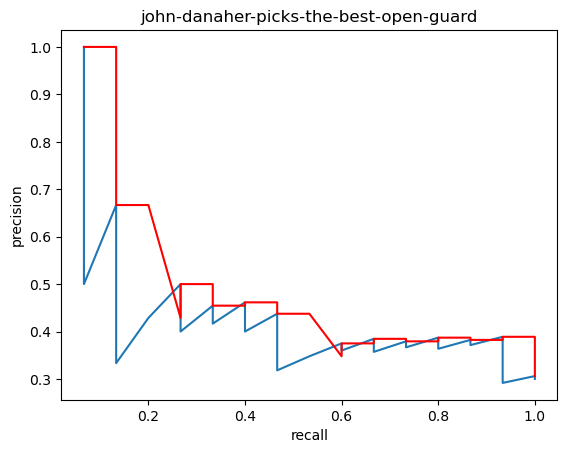
\includegraphics[width=0.5\textwidth]{images/john-danaher-picks-the-best-open-guard_precision-recall.png}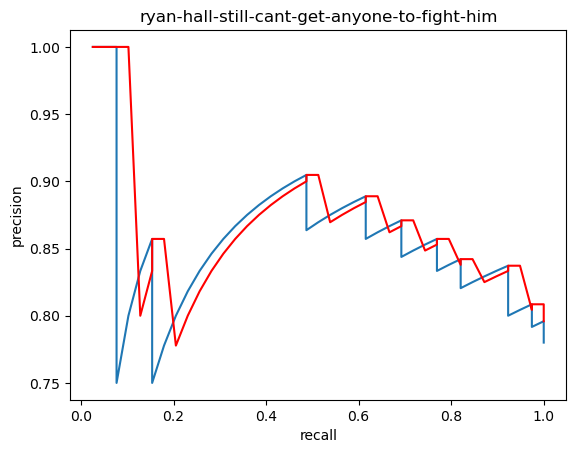
\includegraphics[width=0.5\textwidth]{images/ryan-hall-still-cant-get-anyone-to-fight-him_precision-recall.png} \\
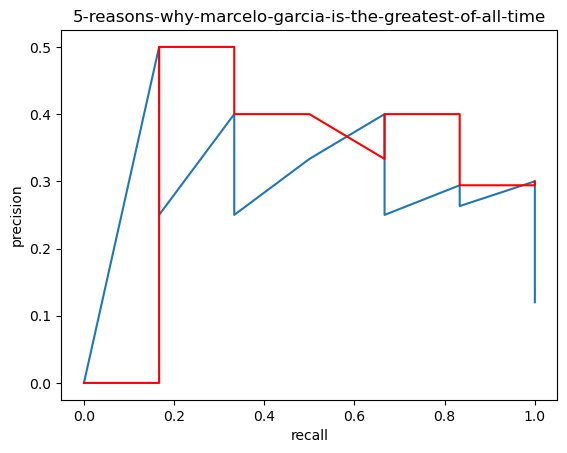
\includegraphics[width=0.5\textwidth]{images/5-reasons-why-marcelo-garcia-is-the-greatest-of-all-time_precision-recall.png}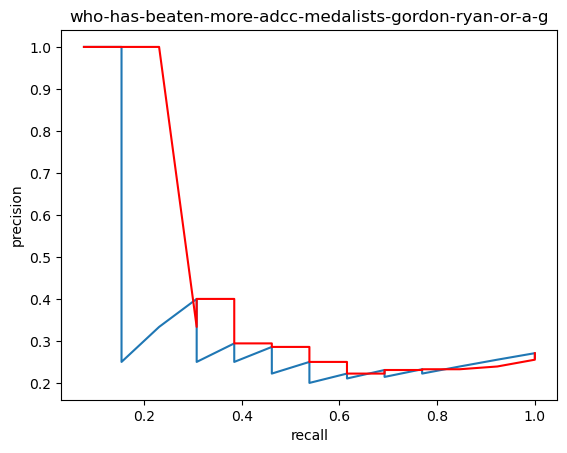
\includegraphics[width=0.5\textwidth]{images/who-has-beaten-more-adcc-medalists-gordon-ryan-or-andre-galvao_precision-recall.png} \\

\noindent Die blaue Linie ist precision@k und recall@k. Die rote Linie ist die beste precision je recall Wert. Bei dieser Auswertung wurde die gegebene Kategorie \texttt{BJJ News} ignoriert, da fast jeder Artikel dieser Kategorie teil ist und somit nahezu ausschlie{\ss}lich true positives zurück kämen. Da unsere Kategorien softe Kategorien sind, sprich sich nicht gegenseitig ausschlie{\ss}en, ist diese Auswertung leider nicht so aussagekräftig wie sie sein könnte.

\subsection{Interpretation}

Die Qualität der zurückgegebenen Dokumente tendiert dazu mit steigendem k abzunehmen, ist jedoch aufgrund der schlechten Kategorien Labels der Webseite so nicht sauber zu evaluieren.

\setcounter{section}{2}
\section{Praktikum 3 - Teil III: Duplikaterkennung mit Shingling und MinHashing}

\subsection{Schritte nachvollziehen}

Aus jedem Dokument wird ein Set von Shingles erstellt und gehasht. Es werden zuerst die Jaccard-Ähnlichkeiten berechnet, dann werden sie mit dem MinHash Algorithmus angewandt.

\subsection{Verbesserungen}

\begin{itemize}
	\item Im vorgegebenen Programm ist die Anzahl der Hash-Funktionen (und dementsprechend die Anzahl der Signaturen) zu klein: Wenn nur 2 Signaturen benutzt werden, dann gibt es nur drei mögliche Werte für EstJ (estimated Jaccard similarity): 1, 0.5, 0. Wenn man stattdessen 3 Signaturen benutzt, dann bekommt man 4 mögliche Werte für EstJ: 1, 0.67, 0.33 und 0.
	\item Zusätzlich kann man den Threshold erhöhen, dann entsteht aber die Gefahr, einige True Positives zu verlieren.
	\item Außerdem kann man die Fenstergröße (i.e., die Anzahl der Wörter in einem Shingle) variieren.
\end{itemize}

\noindent
\textbf{vorher}: \\
\texttt{numHashes}=2, \texttt{window\_length}=3, \texttt{threshold}=0.5 \\
$\Rightarrow$ \texttt{true\_positive}=10, \texttt{false\_positive}=5, \texttt{true\_negative}=985, \texttt{false\_negative=0} \\
$\Rightarrow$ \texttt{precision}=$\frac{2}{3}$, \texttt{recall}=1 \\

\noindent
\textbf{nachher}: \\
\texttt{numHashes}=4, \texttt{window\_length}=3, \texttt{threshold}=0.76 \\
$\Rightarrow$ \texttt{true\_positive}=10, \texttt{false\_positive}=0, \texttt{true\_negative}=990, \texttt{false\_negative}=0 \\
$\Rightarrow$ \texttt{precision}=1, \texttt{recall}=1

\subsection{Zeichenbasiert statt Wortbasiert}

\textbf{zeichenbasiert}: \\
\texttt{numHashes}=4, \texttt{window\_length}=20, \texttt{threshold}=0.5 \\
$\Rightarrow$ \texttt{true\_positive}=10, \texttt{false\_positive}=0, \texttt{true\_negative}=990, \texttt{false\_negative=0} \\
$\Rightarrow$ \texttt{precision}=1, \texttt{recall}=1 \\

\noindent Bei dem zeichenbasierten Shingling dauert die Berechnung der wirklichen Jaccard-Ähnlichkeit sehr lange - 113.3 Sekunden vs. 5.5 Sekunden für das approximative Vorgehen mit den Signaturen (für 1000 Dokumente). Das hat mit der vergrößerten Anzahl von Shingles in jedem Dokument zu tun - durchschnittlich 1560.67 Shingles pro Dokument, wobei es bei dem wortbasierten Shingling nur 251.24 Shingles pro Dokument gab. Wenn man eine deutlich kleinere Fenstergröße nimmt (z.B. 6 Zeichen), dann bekommt man nur eine wenig kleinere Anzahl an Shingles pro Dokument (1432.5), das hat aber - wie erwartet - eine schlechte Auswirkung auf das Ergebnis (30 False Positives).
